% !TEX encoding = UTF-8 Unicode
% REMEMBER TO SET LANGUAGE!
\documentclass[a4paper,10pt,norsk]{article}
\usepackage[utf8]{inputenc}
\usepackage[norsk]{babel}
% Standard stuff
\usepackage{amsmath,graphicx,varioref,verbatim,amsfonts,geometry}
% colors in text
\usepackage[usenames,dvipsnames,svgnames,table]{xcolor}
% Hyper refs
\usepackage[colorlinks]{hyperref}

% Document formatting
\setlength{\parindent}{0mm}
\setlength{\parskip}{1.5mm}

%Color scheme for listings
\usepackage{textcomp}
\definecolor{listinggray}{gray}{0.9}
\definecolor{lbcolor}{rgb}{0.9,0.9,0.9}

%Listings configuration
\usepackage{listings}
%Hvis du bruker noe annet enn python, endre det her for å få riktig highlighting.
\lstset{
	backgroundcolor=\color{lbcolor},
	tabsize=4,
	rulecolor=,
	language=python,
        basicstyle=\scriptsize,
        upquote=true,
        aboveskip={1.5\baselineskip},
        columns=fixed,
	numbers=left,
        showstringspaces=false,
        extendedchars=true,
        breaklines=true,
        prebreak = \raisebox{0ex}[0ex][0ex]{\ensuremath{\hookleftarrow}},
        frame=single,
        showtabs=false,
        showspaces=false,
        showstringspaces=false,
        identifierstyle=\ttfamily,
        keywordstyle=\color[rgb]{0,0,1},
        commentstyle=\color[rgb]{0.133,0.545,0.133},
        stringstyle=\color[rgb]{0.627,0.126,0.941}
        }
        
\newcounter{subproject}
\renewcommand{\thesubproject}{\alph{subproject}}
\newenvironment{subproj}{
\begin{description}
\item[\refstepcounter{subproject}(\thesubproject)]
}{\end{description}}

%Lettering instead of numbering in different layers
%\renewcommand{\labelenumi}{\alph{enumi}}
\renewcommand{\thesubsection}{\alph{subsection}}

%opening
\title{MEK 1100 - Oblig 1}
\author{Joakim Flatby}

\begin{document}

\maketitle

%Oppgave 1
\section{}

Ball kastes ut fra origo.

Utgangsvinkel $\theta$ i forhold til den horisontale x-aksen.

Følger en bane gitt ved:

$x(t) = v_{0} t cos(\theta)$

$y(t) = v_{0} t sin(\theta) - \frac{1}{2}gt^{2}$

%A
\subsection{)}
Finn tiden $t_{m}$ når ballen faller ned på bakken, og posisjonen $x(t_{m}) = x_{m}$ hvor dette skjer:

Når ballen treffer bakken er $y(t) = 0$.

Løser for å finne $t$ ved dette punktet:
\[0 = v_{0} t sin(\theta) - \frac{1}{2}gt^{2}\]
\[\frac{1}{2}gt^{2} = v_{0} t sin(\theta)\]
\[t^{2} = 2\frac{v_{0}tsin(\theta)}{g}\]
\[t_{m} = 2\frac{v_{0}sin(\theta)}{g}\]

Deretter finner vi $x_{m}$ ved å sette uttrykket for $t_{m}$ inn i $x(t)$

\[x(t_{m}) = 2v_{0}\Big( \frac{v_{0}sin(\theta)}{g} \Big) cos(\theta) = \frac{2v_{0}^{2}sin(\theta)cos(\theta)}{g} = \frac{v_{0}^{2}sin(2\theta)}{g}\]

$t_{m} = 2\frac{v_{0}sin(\theta)}{g}$

$x_{m} = \frac{v_{0}^{2}sin(2\theta)}{g}$

%B
\subsection{)}
Innfør dimensjonsløse variabler $(x^{*}, y^{*}, z^{*})$:

\[x^{*} = \frac{x}{x_{m}} = \frac{v_{0}t cos(\theta) * g}{v_{0}^{2} * 2sin(\theta)cos(\theta)} = \frac{gt}{2v_{0}sin(\theta)}\]
\\ \\
\[y^{*} = \frac{y}{x_{m}} = \frac{(v_{0}t sin(\theta) - \frac{1}{2}gt^{2}) * g}{v_{0}^{2} * 2sin(\theta)cos(\theta)} = \frac{v_{0} * g t sin(\theta)}{v_{0}^{2} * 2sin(\theta)cos(\theta)} - \frac{\frac{1}{2}gt^{2} * g}{v_{0}^{2} * 2sin(\theta)cos(\theta)}\]
\[y^{*} = \frac{gt}{v_{0} * 2cos(\theta)} - \frac{g^{2}t^{2}}{v_{0}^{2} * 4sin(\theta)cos(\theta)}\]
\[y^{*} = \frac{gt}{2v_{0}cos(\theta)} * \Big(1 - \frac{gt}{2v_{0}sin(\theta)}\Big)\]
$\frac{gt}{2v_{0}sin(\theta)} = x^{*}$
\[y^{*} = \frac{gt}{2v_{0}cos(\theta)} * (1 - x^{*})\]
\[y^{*} = \frac{gt}{2v_{0}cos(\theta)} * \frac{sin(\theta)}{sin(\theta)} * (1 - x^{*})\]
\[y^{*} = x^{*}tan(\theta)(1 - x^{*})\]
\\ \\
\[t^{*} = \frac{t}{t_{m}} = \frac{tg}{2v_{0}sin(\theta)} = x^{*}\]

Ettersom $\theta$ beskrives ved å ta $\frac{buelengde}{radius}$, og dette ikke har noen benevning: $\Big[\frac{avstand}{avstand}\Big] = 1$, så trenger ikke $\theta$ å skaleres.

%C
\subsection{)}

\lstinputlisting{oppg1.py}

\begin{figure}[h!]
        \centering 
        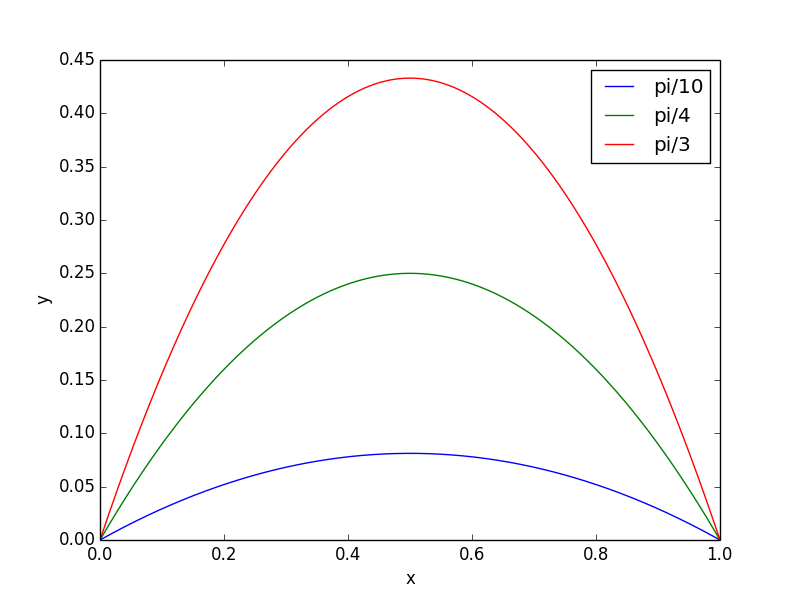
\includegraphics[scale=0.5]{oppg1.png} 
        \caption{PyPlot, plotter x* og y* for 3 forskjellige verdier for $\theta$}
\end{figure}

Ved å se på denne grafen ser vi forholdet mellom høyden og lengden på banen ved forskjellige verdier av utfallsvinkelen $\theta$. 
Verdiene kan brukes for alle verdier av $g$ og $v_{0}$ fordi $x^{*}$ er dimensjonsløs, og $\theta$ er den eneste variablen vi bruker for å beskrive grafen.

%Oppgave 2
\section{}

Hastighetsfeltet: $\vec{v} = v_{x}\vec{i} + v_{y}\vec{j} = xy\vec{i} + y\vec{j}$

%A
\subsection{)}
Finn strømlinjene:

Ser på kryssproduktet $\vec{v} \times d\vec{r}$, som gir 0 ettersom $\vec{v}$ og $d\vec{r}$ er parallelle.

Da får vi:

\[(v_{x}dy - vydx)\vec{k} = 0\]
\[v_{x}dy = v_{y}dx\]
\[xydy = ydx\]
Deler på $xy$:
\[1dy = \frac{1}{x}dx\]
\[\int 1 dy = \int frac{1}{x}dx\]
\[y = ln|x| + C\]
\[C = y - ln|x|\]

%B
\subsection{)}

\begin{figure}[h!]
        \centering 
        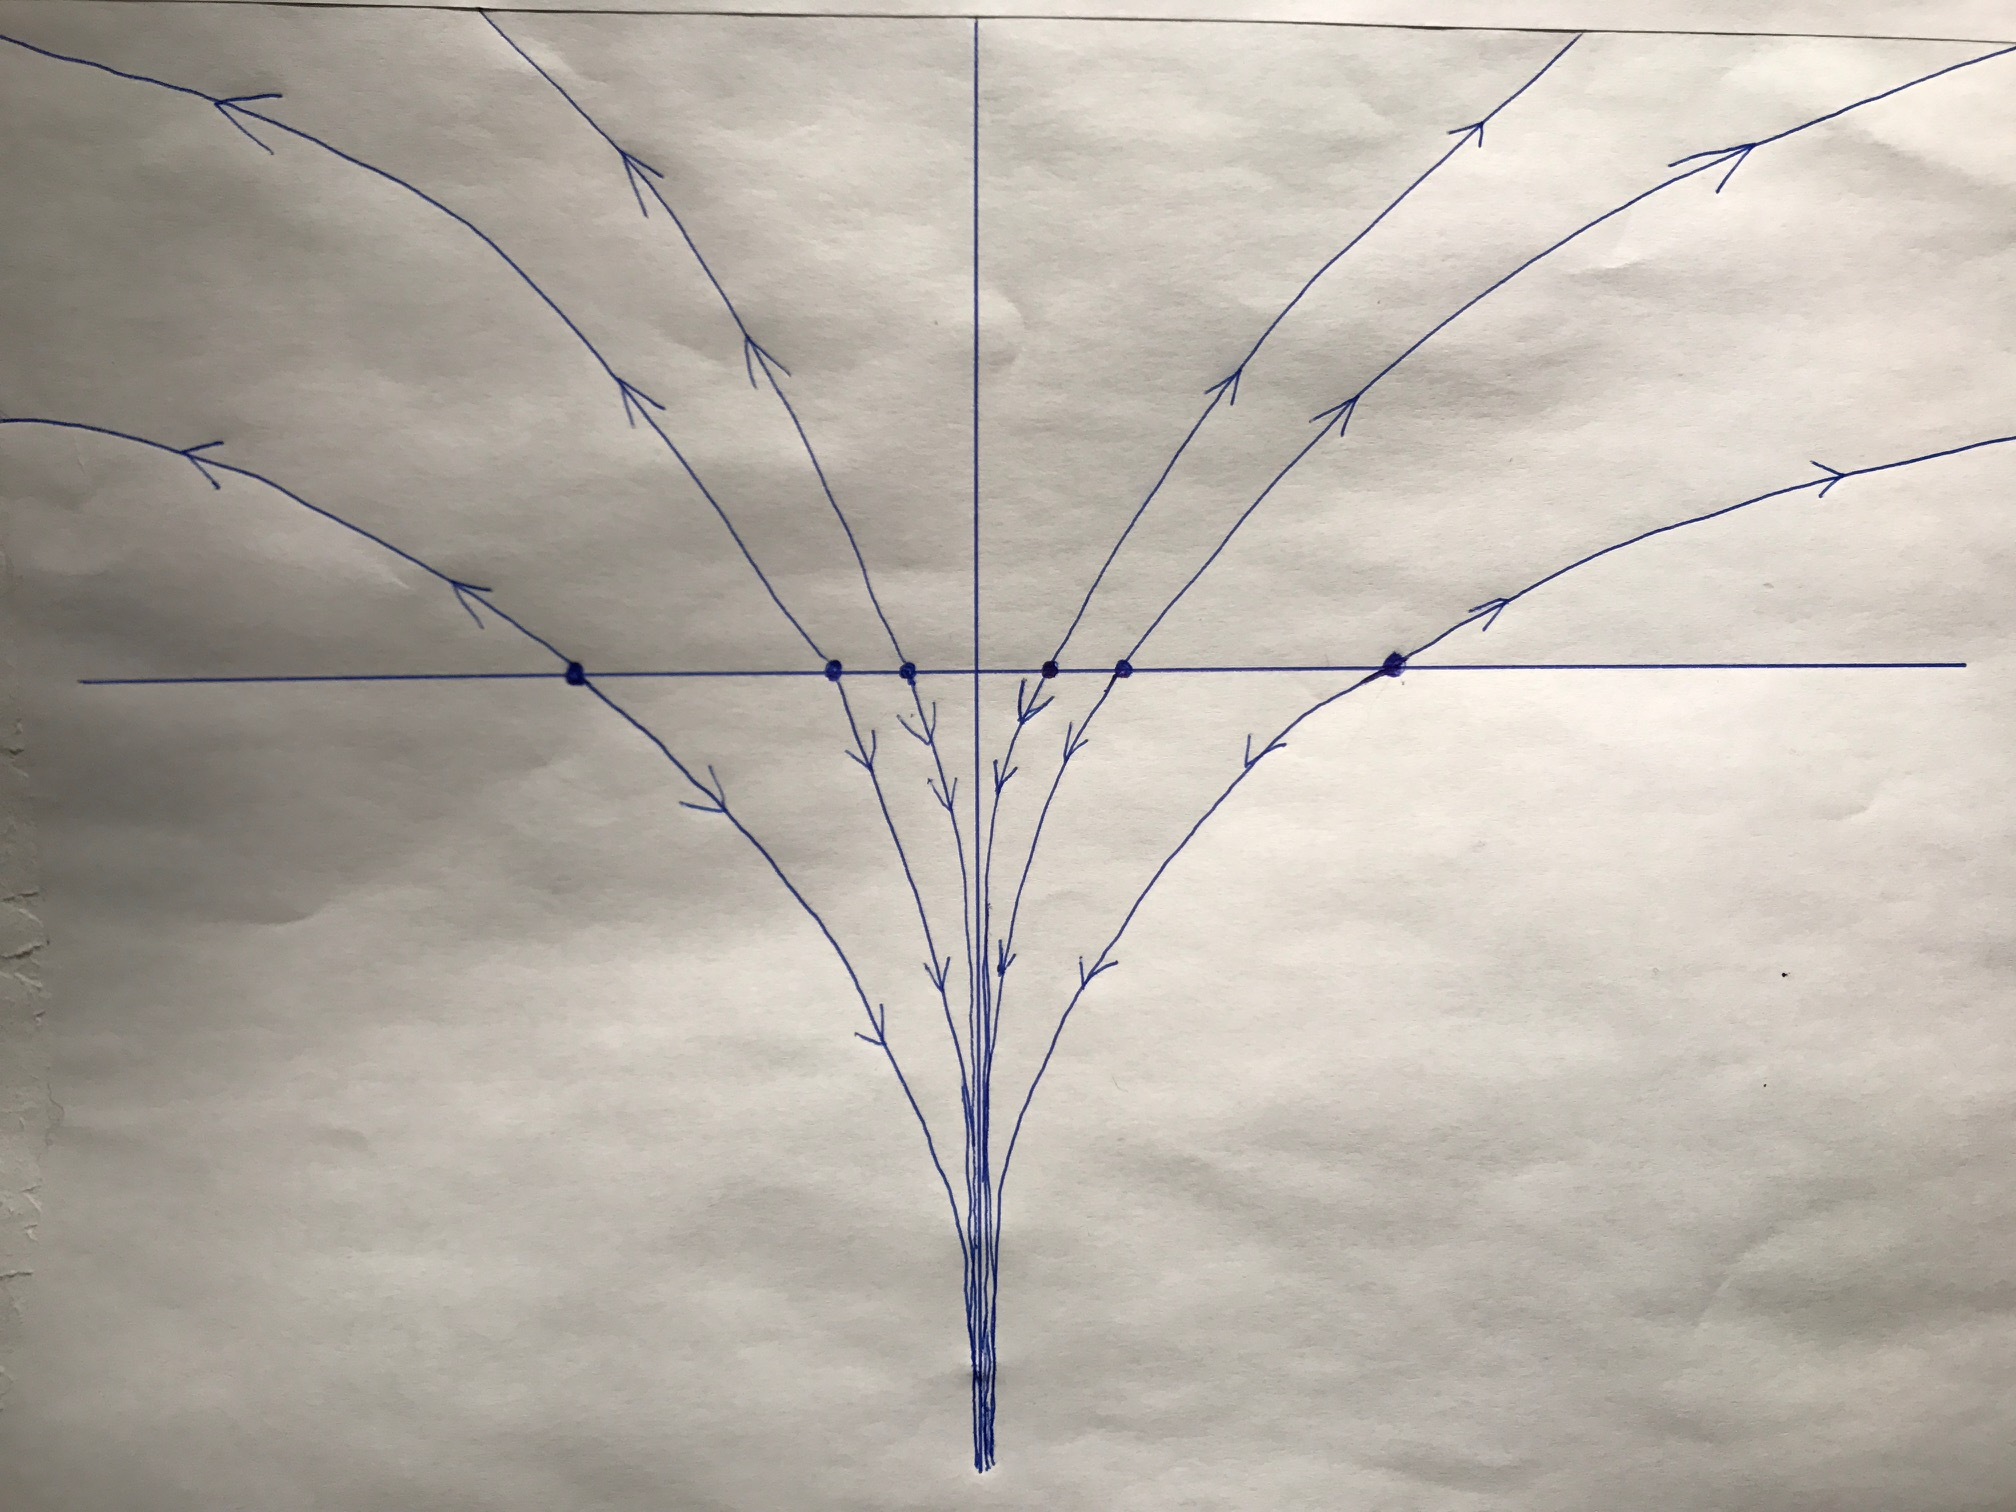
\includegraphics[scale=0.2]{stromlinjer.jpg} 
\end{figure}

\lstinputlisting{oppg2.py}

\begin{figure}[h!]
        \centering 
        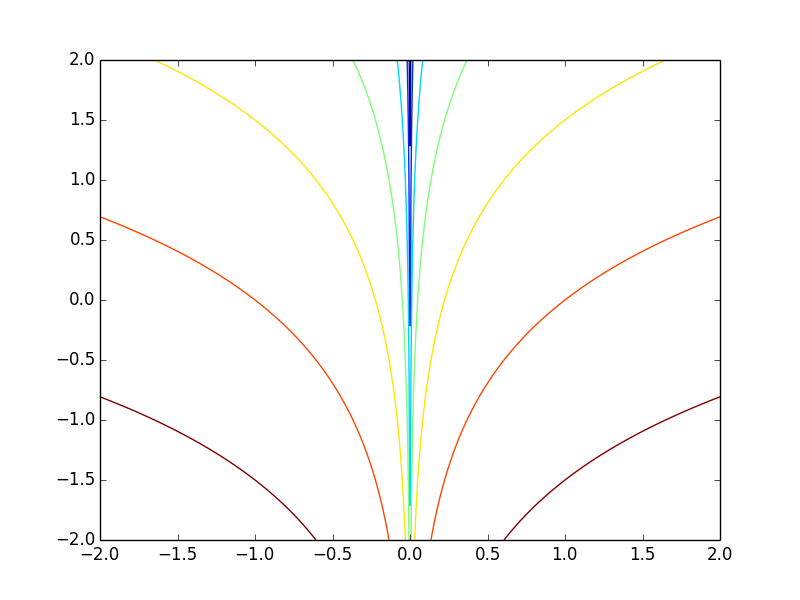
\includegraphics[scale=0.6]{oppg2.png} 
\end{figure}

%C
\subsection{)}
Vis at det $\bold{ikke}$ finnes en strømfunksjon $\psi$:

\[\frac{\delta(v_{x})}{\delta x} + \frac{\delta(v_{y})}{\delta y} = \frac{\delta(xy)}{\delta x} + \frac{\delta y}{\delta y} = y + 1\]
\[y + 1 \neq 0\]
Feltet er ikke divergens-fritt, så dermed har det ingen strømfunksjon.

%oppgave 3
\section{}

$v_{x} = cos(x) sin(y)$

$v_{y} = -sin(x) cos(y)$

%A
\subsection{)}
Finn divergens og virvling.

Divergens:
\[\frac{\delta(v_{x})}{\delta x} + \frac{\delta(v_{y})}{\delta y}\]
$\frac{\delta(v_{x})}{\delta x} = \frac{\delta(cos(x)sin(y))}{\delta x} = \frac{1}{2}cos(x + y) - \frac{1}{2}cos(x - y)$

$\frac{\delta(v_{y})}{\delta y} = \frac{\delta(-sin(x)cos(y))}{\delta y} = \frac{1}{2}cos(x - y) - \frac{1}{2}cos(x +y)$
\[\frac{1}{2}cos(x + y) - \frac{1}{2}cos(x - y) + \frac{1}{2}cos(x - y) - \frac{1}{2}cos(x +y) = 0\]

Virvling:
\[\Big(\frac{\delta(v_{y})}{\delta x} - \frac{\delta(v_{x})}{\delta y}\Big) \vec{k}\]
\[\frac{\delta(v_{y})}{\delta x} = \frac{\delta(-sin(x)cos(y))}{\delta x} = -cos(x)cos(y)\]
\[\frac{\delta(v_{x})}{\delta y} = \frac{\delta(cos(x)sin(x))}{\delta y} = cos(x)cos(y)\]

\[= \Big(-cos(x) cos(y) - cos(x)cos(y)\Big)\vec{k}\]
\[= \Big(-2cos(x)cos(y) \Big) \vec{k}\]


%B
\subsection{)}

\begin{figure}[h!]
        \centering 
        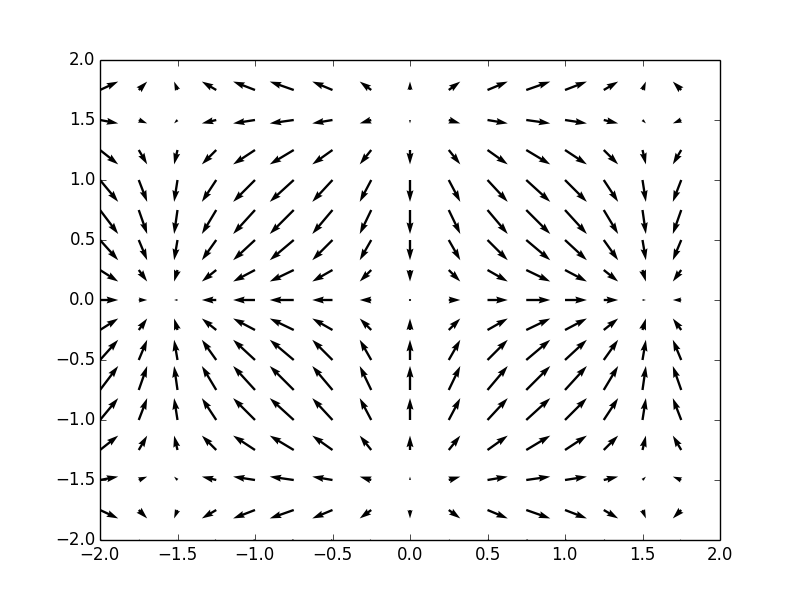
\includegraphics[scale=0.7]{oppg3.png}
\end{figure}

\lstinputlisting{oppg3.py}



%C
\subsection{)}
Integrerer hastighetsfeltet over et kurveintegral ved å dele opp kurven i fire sider med parametriseringen $\vec{r_{i}}$ hvor $i$ er siden vi ser på.

Bruker formelen: 
\[\int \vec{v}d\vec{r_{i}} = \int_{a}^{b}\vec{v}(\vec{r_{i}}(t)) * \vec{r_{i}}'dt\]
med $a = -\frac{\pi}{2}$ og $b = \frac{\pi}{2}$

Ser på parameterene:
\[\vec{r_{1}}(t) = (t, -\frac{\pi}{2}) \Rightarrow \vec{r_{1}}'(t) = (1, 0)\]
\[\vec{r_{2}}(t) = (\frac{\pi}{2}, t) \Rightarrow \vec{r_{2}}'(t) = (0, 1)\]
\[\vec{r_{3}}(t) = (-t, \frac{\pi}{2}) \Rightarrow \vec{r_{3}}'(t) = (-1, 0)\]
\[\vec{r_{4}}(t) = (-\frac{\pi}{2}, -t) \Rightarrow \vec{r_{4}}'(t) = (0, -1)\]

Bruker deretter formelen og regner ut $\int_{a}^{b} \vec{v}(\vec{r_{i}}(t)) * \vec{r_{i}}'dt$ for alle sider $i$:
\[\int_{-\frac{\pi}{2}}^{\frac{\pi}{2}}\vec{v}(\vec{r_{1}}(t)) * \vec{r_{1}}'dt = \int_{-\frac{\pi}{2}}^{\frac{\pi}{2}}cos(t)sin\Big(\frac{\pi}{2}\Big) dt = \Big[-sin(t)\Big]_{-\frac{\pi}{2}}^{\frac{\pi}{2}} = -2\]
\[\int_{-\frac{\pi}{2}}^{\frac{\pi}{2}}\vec{v}(\vec{r_{2}}(t)) * \vec{r_{2}}'dt = \int_{-\frac{\pi}{2}}^{\frac{\pi}{2}}-sin\Big(\frac{\pi}{2}\Big) cos(t) dt = \Big[-sin(t)\Big]_{-\frac{\pi}{2}}^{\frac{\pi}{2}} = -2\]
\[\int_{-\frac{\pi}{2}}^{\frac{\pi}{2}}\vec{v}(\vec{r_{3}}(t)) * \vec{r_{3}}'dt = \int_{-\frac{\pi}{2}}^{\frac{\pi}{2}}-cos(-t)sin\Big(\frac{\pi}{2}\Big) dt = \Big[sin(-t)\Big]_{-\frac{\pi}{2}}^{\frac{\pi}{2}} = -2\]
\[\int_{-\frac{\pi}{2}}^{\frac{\pi}{2}}\vec{v}(\vec{r_{4}}(t)) * \vec{r_{4}}'dt = \int_{-\frac{\pi}{2}}^{\frac{\pi}{2}}-sin\Big(-\frac{\pi}{2}\Big) cos(-t) dt = \Big[sin(-t)\Big]_{-\frac{\pi}{2}}^{\frac{\pi}{2}} = -2\]

Ettersom summen av disse blir $-8$, er sirkulasjonen om randen til kvadratet $-8$

%D
\subsection{)}
Dette feltet er divergensfritt(i motsetning til forrige oppgave), og dermed så har feltet en strømfunksjon.

\[cos(x)sin(y) = -\frac{\delta\psi}{\delta y}\]
\[\int -cos(x)sin(y) dy = \int \frac{\delta \psi}{\delta y}\]
\[-cos(x)\int sin(y)dy = \psi\]
\[\psi = cos(x)cos(y) + C_{1}\]

\[-sin(x)cos(y) = \frac{\delta\psi}{\delta x}\]
\[\int -sin(x)cos(y)dx = \int\frac{\delta \psi}{\delta x}\]
\[-cos(y) \int sin(x)dx = \psi\]
\[\psi = cos(x)cos(y) + C_{2}\]

Dermed får vi:
\[\psi = cos(x)cos(y)\]


%E
\subsection{)}
\[\psi(x, y) \approx \psi(x_{0}, y_{0}) + \Big(\frac{\delta \psi}{\delta x}\Big)(x-x_{0}) + \Big(\frac{\delta \psi}{\delta y}\Big)(y-y_{0})+ \Big(\frac{\delta^{2} \psi}{2\delta x^{2}}\Big)(x-x_{0})^{2} + \Big(\frac{\delta^{2} \psi}{2\delta y^{2}}\Big)(y - y_{0})^{2} + \Big(\frac{\delta^{2}\psi}{\delta x \delta y}\Big)(x-x_{0})(y-y_{0})\]

\[\frac{\delta \psi}{\delta x} = -sin(x) cos(y), \ \frac{\delta \psi}{\delta x}(0, 0) = 0 \]
\[\frac{\delta \psi}{\delta y} = -cos(x) sin(y), \ \frac{\delta \psi}{\delta x}(0, 0) = 0 \]
\[\frac{\delta^{2} \psi}{\delta x^{2}} = -cos(x) cos(y), \ \frac{\delta \psi}{\delta x}(0, 0) = -1 \]
\[\frac{\delta^{2} \psi}{\delta y^{2}} = -cos(x) cos(y), \ \frac{\delta \psi}{\delta x}(0, 0) = -1 \]
\[\frac{\delta^{2} \psi}{\delta x \delta y} = -sin(x) sin(y), \ \frac{\delta \psi}{\delta x}(0, 0) = 0 \]

Setter dette inn i formelen over for å få taylorekspansjonen.

\[\psi(0, 0) \approx \psi(0, 0) + \Big(\frac{\delta \psi}{\delta x}\Big) x + \Big(\frac{\delta \psi}{\delta y}\Big) y + \Big(\frac{\delta^{2} \psi}{2\delta x^{2}}\Big) x^{2} + \Big(\frac{\delta^{2} \psi}{2\delta y^{2}}\Big) y^{2} + \Big(\frac{\delta^{2}\psi}{\delta x \delta y}\Big) xy\]
\[ = 1 + 0 + 0 - \frac{x^{2}}{2} - \frac{y^{2}}{2}\]
\[ = 1 - \frac{x^{2} - y^{2}}{2}\]

\pagebreak

%Oppgave 4
\section{}

%A
\subsection{)}

\begin{figure}[h!]
        \centering 
        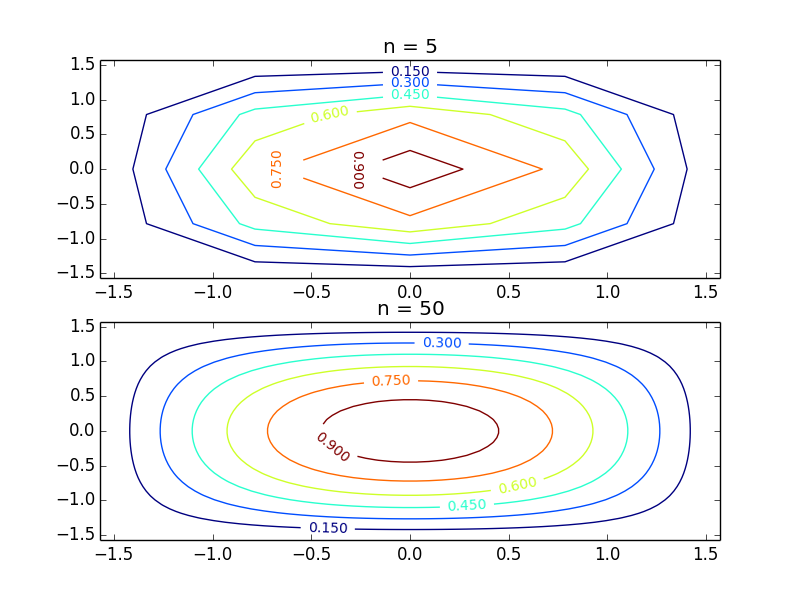
\includegraphics[scale=0.7]{strlin.png} 
\end{figure}

\lstinputlisting{strlin.py}

\pagebreak

%B
\subsection{)}

Valgte n=10 for å få passende lesbarhet av plottet.

\begin{figure}[h!]
        \centering 
        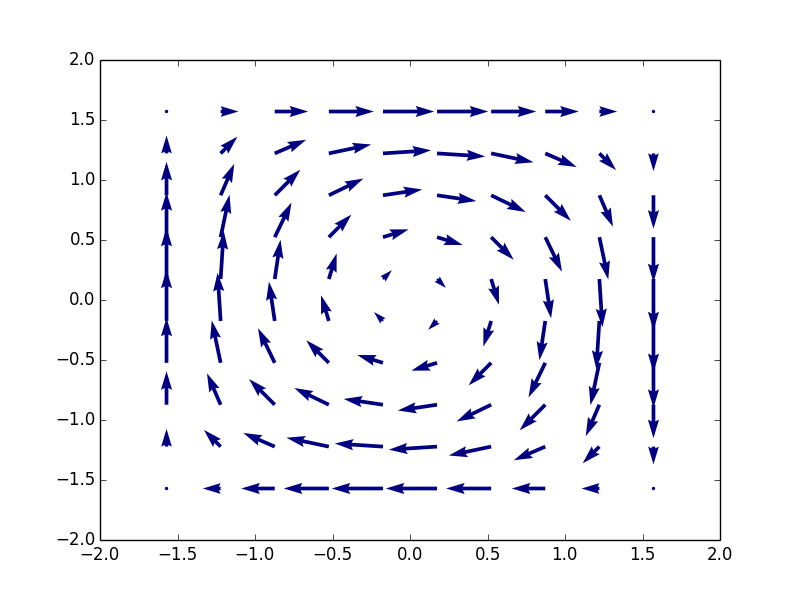
\includegraphics[scale=0.7]{velfield.png} 
\end{figure}

\lstinputlisting{velfield.py}

\lstinputlisting{vec.py}

\end{document}

